\chapter{Another chapter}\label{ch:results}

\section{Ground State Degeneracy}
In this chapter results of simulations on the dipolar kagome lattice are presented. EFM simulations reveal zero-temperature states lacking domain walls that consist of 3 spins and their negatives. Every ground state obtained through the EFM simulation exhibits a three-sublattice structure with one spin and its negative for each sublattice. The spins alternate in direction along the [1,1,1] direction. 

\begin{figure}
	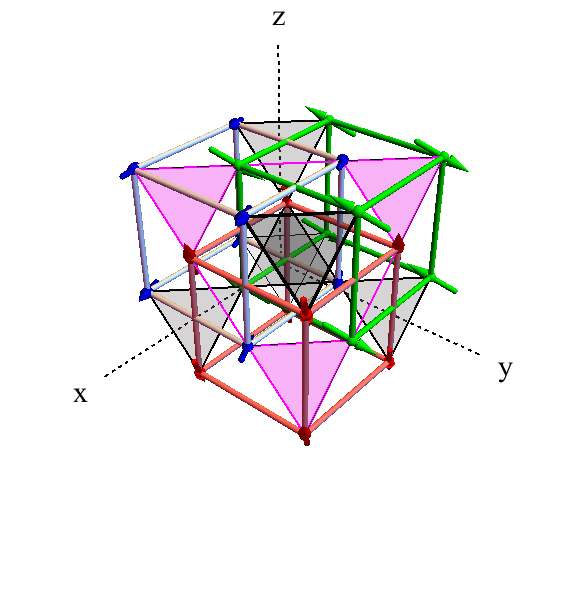
\includegraphics[width=\linewidth]{img/3dfcc.png}
	\caption{A view down the <1,1,1> axis of a 3D FCC lattice with six sub-lattice spin vectors.}
	\label{fig:3dfcc}
\end{figure}

\clearpage
Every ground state configuration obtained through the EFM simulation is characterized by the following set of equations:
\begin{equation}
\label{eqn:rel_a}
\alpha = \sin{\theta} \cos{\phi}
\end{equation}
\begin{equation}
\label{eqn:rel_b}
\beta = \sin{\theta} \sin{\phi}
\end{equation}
\begin{equation}
\label{eqn:rel_c}
\chi = \cos{\theta}
\end{equation}
\begin{equation}
\label{eqn:rel_d}
\delta = (2a^2-1)/2c
\end{equation}
\begin{equation}
\label{eqn:rel_e}
\epsilon = \sqrt(1-a^2-d^2)
\end{equation}

This set of equations acts as elementary building blocks for the components of the spin vectors that exist in the dipolar kagome ground state. The spin vectors may be constructed with this set of equations using the following configuration.

$$\overrightarrow{a} = (\alpha, \beta, \chi)$$
$$\overrightarrow{b} = (\delta, \epsilon, -\alpha)$$
$$\overrightarrow{c} = (-\epsilon, -\chi-\delta, \beta)$$
$$\overrightarrow{d} =-\overrightarrow(a)$$
$$\overrightarrow{e} =-\overrightarrow(b)$$
$$\overrightarrow{f} =-\overrightarrow(c)$$


The set of all possible ground states is therefore characterizable in terms of two parameters: theta and phi. Any theta and phi gives rise to an acceptable ground state of the same energy for a particular lattice size, with the exception of a subset of angles that results in imaginary values for the spin components or undefined division by zero.

\begin{figure}
	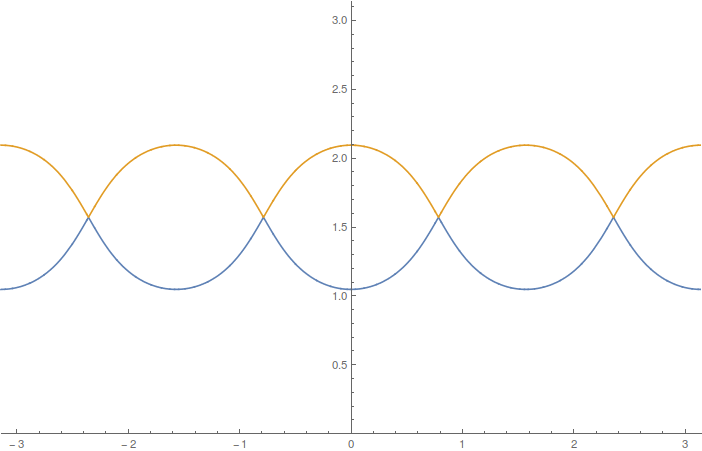
\includegraphics[width=\linewidth]{img/degeneracyplanefull.png}
	\caption{A plane that contains points that allow the construction of valid ground states.}
	\label{fig:degenplanefull}
\end{figure}


Any theta and phi will give rise to a valid ground state of the same energy with the exception of those pairs of theta and phi that lie within the bound region of the graph. Within the bound region of the graph, e = √(1–a²–d²) ∈ ℂ. At each node of each bound area, d = (2a²–1)/2c → ±0/0. Therefore, any choice of theta and phi outside of this region will give rise to a valid ground state of the same energy.

\begin{figure}
	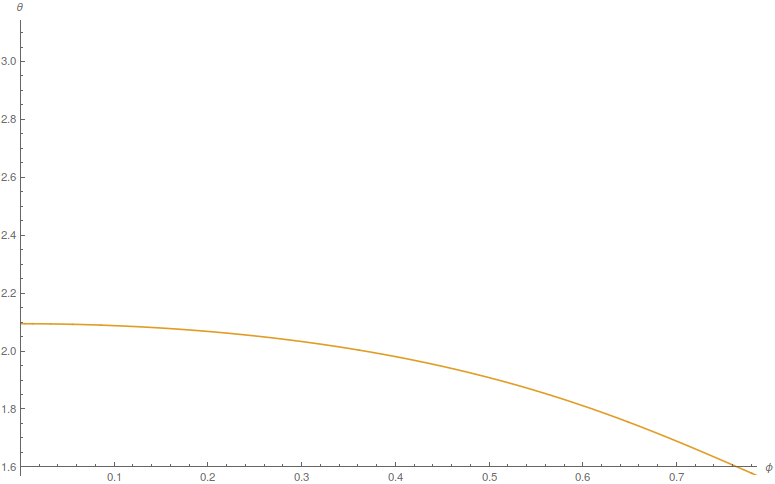
\includegraphics[width=\linewidth]{img/degeneracyplane.png}
	\caption{One section of the original degeneracy plane that is equivalent to all other sections of the plane due to symmetry operations.}
	\label{fig:degenplane}
\end{figure}

It is possible to reduce the size of this graph to 1/16 the size by showing that a state in each portion of the graph is relatable to an analogous state in the other portions of the graph via symmetry operations.
\clearpage

\subsection{Visualization of the Ground State}
\begin{center}
\begin{figure}[ht]
	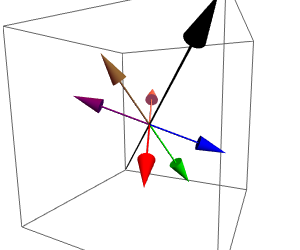
\includegraphics[scale=1.2]{img/samplegs.png}
	\caption{The six sublattice spins conjoined at their ends for clarity and illustration. The vector denoting <1,1,1> axis of symmetry is illustrated in black}
	\label{fig:sampgs}
\end{figure}
\end{center}

By generating the spin vectors described by the !!!equations!!!, a variety of spin configurations can b
\clearpage